%%%%%%%% ICML 2018 EXAMPLE LATEX SUBMISSION FILE %%%%%%%%%%%%%%%%%

\documentclass{article}

% Recommended, but optional, packages for figures and better typesetting:
\usepackage{amstext}
\usepackage{microtype}
\usepackage{graphicx}
\usepackage{subfigure}
\usepackage{tikz}
\usepackage{booktabs} % for professional tables

\usetikzlibrary {positioning}
\usepackage{graphicx,caption}

\usepackage{subcaption}
\definecolor {processblue}{cmyk}{0.96,0,0,0}

\usepackage[T1]{fontenc} 
\usepackage[utf8]{inputenc}
\pagenumbering{roman}

% hyperref makes hyperlinks in the resulting PDF.
% If your build breaks (sometimes temporarily if a hyperlink spans a page)
% please comment out the following usepackage line and replace
% \usepackage{icml2018} with \usepackage[nohyperref]{icml2018} above.
\usepackage{hyperref}

% Attempt to make hyperref and algorithmic work together better:
\newcommand{\theHalgorithm}{\arabic{algorithm}}

% Use the following line for the initial blind version submitted for review:
% \usepackage{icml2018}

% If accepted, instead use the following line for the camera-ready submission:
\usepackage[accepted]{icml2018}

% The \icmltitle you define below is probably too long as a header.
% Therefore, a short form for the running title is supplied here:
\icmltitlerunning{Neural mechanisms of risk-sensitive choice and reinforcement
learning under uncertainty}

\newcommand{\keyword}[1]{\textit{#1}}

\begin{document}

\twocolumn[
\icmltitle{Neural mechanisms of risk-sensitive choice and reinforcement
learning under uncertainty}

% It is OKAY to include author information, even for blind
% submissions: the style file will automatically remove it for you
% unless you've provided the [accepted] option to the icml2018
% package.

% List of affiliations: The first argument should be a (short)
% identifier you will use later to specify author affiliations
% Academic affiliations should list Department, University, City, Region, Country
% Industry affiliations should list Company, City, Region, Country

% You can specify symbols, otherwise they are numbered in order.
% Ideally, you should not use this facility. Affiliations will be numbered
% in order of appearance and this is the preferred way.

\begin{icmlauthorlist}
\icmlauthor{Emil Azadian}{equal,tu}
\icmlauthor{Jan Botsch}{equal,tu}
\icmlauthor{Vlad-Catalin Frasineanu}{equal,tu}
\icmlauthor{Oğuz Şerbetci}{equal,tu}
\icmlauthor{Stephan Tietz}{equal,tu}
\end{icmlauthorlist}

\icmlaffiliation{tu}{TU Berlin, Neural Information Processing Group}

\icmlcorrespondingauthor{Emil Azadian}{oguz.serbetci@campus.tu-berlin.de}
\icmlcorrespondingauthor{Jan Botsch}{oguz.serbetci@campus.tu-berlin.de}
\icmlcorrespondingauthor{Vlad-Catalin Frasineanu}{oguz.serbetci@campus.tu-berlin.de}
\icmlcorrespondingauthor{Oğuz Şerbetci}{oguz.serbetci@campus.tu-berlin.de}
\icmlcorrespondingauthor{Stephan Tietz}{stietz@campus.tu-berlin.de}

% You may provide any keywords that you
% find helpful for describing your paper; these are used to populate
% the "keywords" metadata in the PDF but will not be shown in the document
\icmlkeywords{Machine Learning, Reinforcement Learning, Risk Sensitivity}

\vskip 0.3in
]

% this must go after the closing bracket ] following \twocolumn[ ...

% This command actually creates the footnote in the first column
% listing the affiliations and the copyright notice.
% The command takes one argument, which is text to display at the start of the footnote.
% The \icmlEqualContribution command is standard text for equal contribution.
% Remove it (just {}) if you do not need this facility.

% \printAffiliationsAndNotice{}  % leave blank if no need to mention equal contribution
\printAffiliationsAndNotice{\icmlEqualContribution} % otherwise use the standard text.

\begin{abstract}
\textit{Utility functions are often used to explain human risk behaviour under uncertainty. We present a class of reinforcement learning agents trained on different utility functions that are able to mimic risky choice under uncertainty. We use self-gathered experimental data capturing risk profiles of human participants and apply the agent's results to them. From that, we deduct that the widely used exponential utility function might not be able to explain all human risk profiles. In turn, we present two other utility functions that could be suited for mapping risk profiles.}
\end{abstract}

\section{Introduction}\label{sec:introduction}
In our everyday lives we are forced to act under uncertainty, meaning in circumstances where we do not have full information. Imagine for example that you want to catch the local bus to university. You know when it is supposed to arrive, but it could very well be that the bus is a couple of minutes early or late - there is uncertainty involved. How we act under uncertainty is an indicator of our risk profile: Some people will want to avoid the risk of missing the bus and decide to leave for the station rather early, others might speculate that the bus will be late and leave accordingly, expressing a more risky behaviour. This behaviour is called the risk profile or risk-sensitivity of a person.\\
It has long been a goal of economics to capture risk profiles in a consistent manner. This paper will use a Machine Learning approach to reassess one of the theories that are used by economists to explain risk sensitivity, namely the use of utility functions.

\section{Background}\label{sec:background}
\subsection{Measuring risk}

Measuring risk and peoples behaviour under risky choice is a much debated topic in economics. In purely financial contexts variance is often used as a proxy for risk. Options with high variance are considered more risky than options with lower variance. 
A decision maker would therefore calculate the expected return and the corresponding variance of each option available.
Then if one option has lower risk and higher expected return than the other it is said to be dominant and should be preferred.
This model has some shortfalls, i.e. it is easy to construct cases where empirical studies clearly show that it is not sufficient to explain human behaviour.
% More complex measures have been introduced to explain these behaviours like Value At Risk, semi-variance (splitting variance into losses and gains) and expected shortfall. But all of these are highly abstract and would require quite some effort to evaluate as variance is hard to estimate. 
It can therefore be assumed that this hardly describes peoples everyday risk behaviour, instead a simpler and more intuitive way is required. \cite{Jaeger00}
% add example

Two mathematicians, Von Neumann and Morgenstern, gave rise to a method more useful for describing individuals behaviour. They postulated in the 1950s that when facing a risky decision people will maximize not their expected value but their expected utility. \cite{Morgenstern53}
The theory is therefore called expected utility theory. \cite{Grant07}
To every possible outcome one assigns a utility value as defined by a real valued utility function. The person does not need to know (and most likely doesn't know) about their utility function. They will implicitly assign utilities and then pick the option that maximizes their expected function value.


\begin{figure}[ht]
\centering
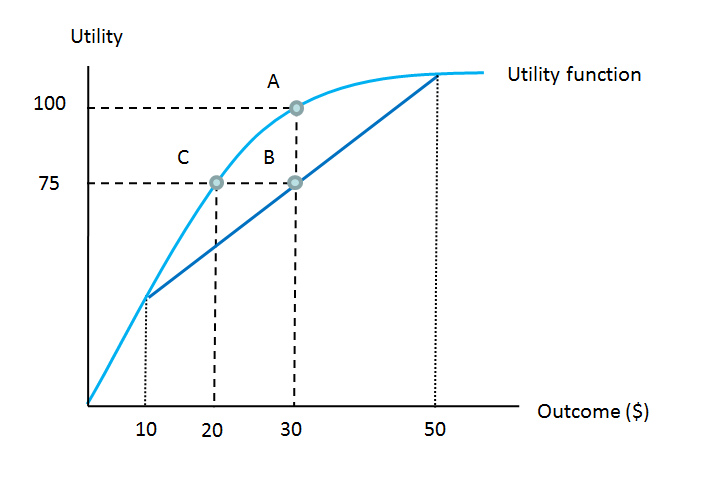
\includegraphics[width=0.5\textwidth]{img/background/riskaversion}%
\caption{Choice from a risk free gift of 30\$ or a lottery where by coin flip you win 10\$ or 50\$. The utility for the risk free choice (point A) is higher than the expected utility of the risky lottery (point B). Figure taken from \cite{pic_risk}. 
% b) The exponential utility function for different risk parameters $\lambda$. $\lambda < 0$ implies risk seeking, $\lambda = 0 $ risk neutral and $\lambda > 0 $ risk averse behaviour.
}
\label{fig:background:riskaversion}
\end{figure}


To illustrate this we will look at the example illustrated in figure \ref{fig:background:riskaversion}:
A person is asked to choose from a gift of 30\$ or to participate in a fair coin flip where she can win 10\$ or 50\$.
It's easy to see that the expected outcome for both options is 30\$ but the coin flip is risky while the gift is risk free.
The person in figure \ref{fig:background:riskaversion} acts in line with a concave risk function, i.e. in the limit the utility grows slower than the outcome. This also leads to a saturation effect where higher values are valued less and less which can often be observed in economics. %https://books.google.de/books?id=II4Nwm1uoCIC&pg=PA156&lpg=PA156&dq=utility+saturation+effect&source=bl&ots=HTlYRm8HtH&sig=jlqdH5UPyURI-SWXYlCJ5DzWXsY&hl=de&sa=X&ved=2ahUKEwjL-cHox8bcAhWPZlAKHVj3DHMQ6AEwAXoECAEQAQ#v=onepage&q=utility%20saturation%20effect&f=false
The utility assigned to the possible outcome of 10\$ is around 40, the utility for 50\$ around 110 (both indicated by the dotted vertical lines). The expected utility of the coin flip (for different unfair coins) is simply the linear interpolation in between these two points. As we are using a fair coin the expected utility is right in the middle marked with the letter B at 75. In comparison the expected utility for the gift of 30\$ is at 100, indicated by letter A. The person in this example would therefore prefer the risk free choice of the gift over the risky coin flip.


\textbf{It is an important observation that concave utility functions describe risk averse decision makers whereas convex utility functions describe risk seeking decision makers. }

Different risk profiles can therefore be modelled by differently curved utility functions. Note that the curvature does not need to remain the same over all outcomes but can change, allowing to model risk seeking behaviour in some realm, e.g. for small amounts of money and risk averse behaviour in others, e.g. loss of life.

A very common and easy to parametrize utility function is the exponential function defined as:
\begin{flalign}
& U(w)  =  
\begin{cases}
	\frac{1-\exp(- \lambda w)}{\lambda} & \lambda \neq 0\\
	w & \lambda = 0
	\label{equ:exp}
\end{cases}
\end{flalign}
It is often chosen for its mathematical convenience yet its applicability is highly questionable as it implies time independent decisions, i.e. past losses are not considered when making new decisions. The impact of the parameter $\lambda$ on the curvature of the function is shown in figure \ref{fig:background:exponential}. 

\begin{figure}[ht]
\centering
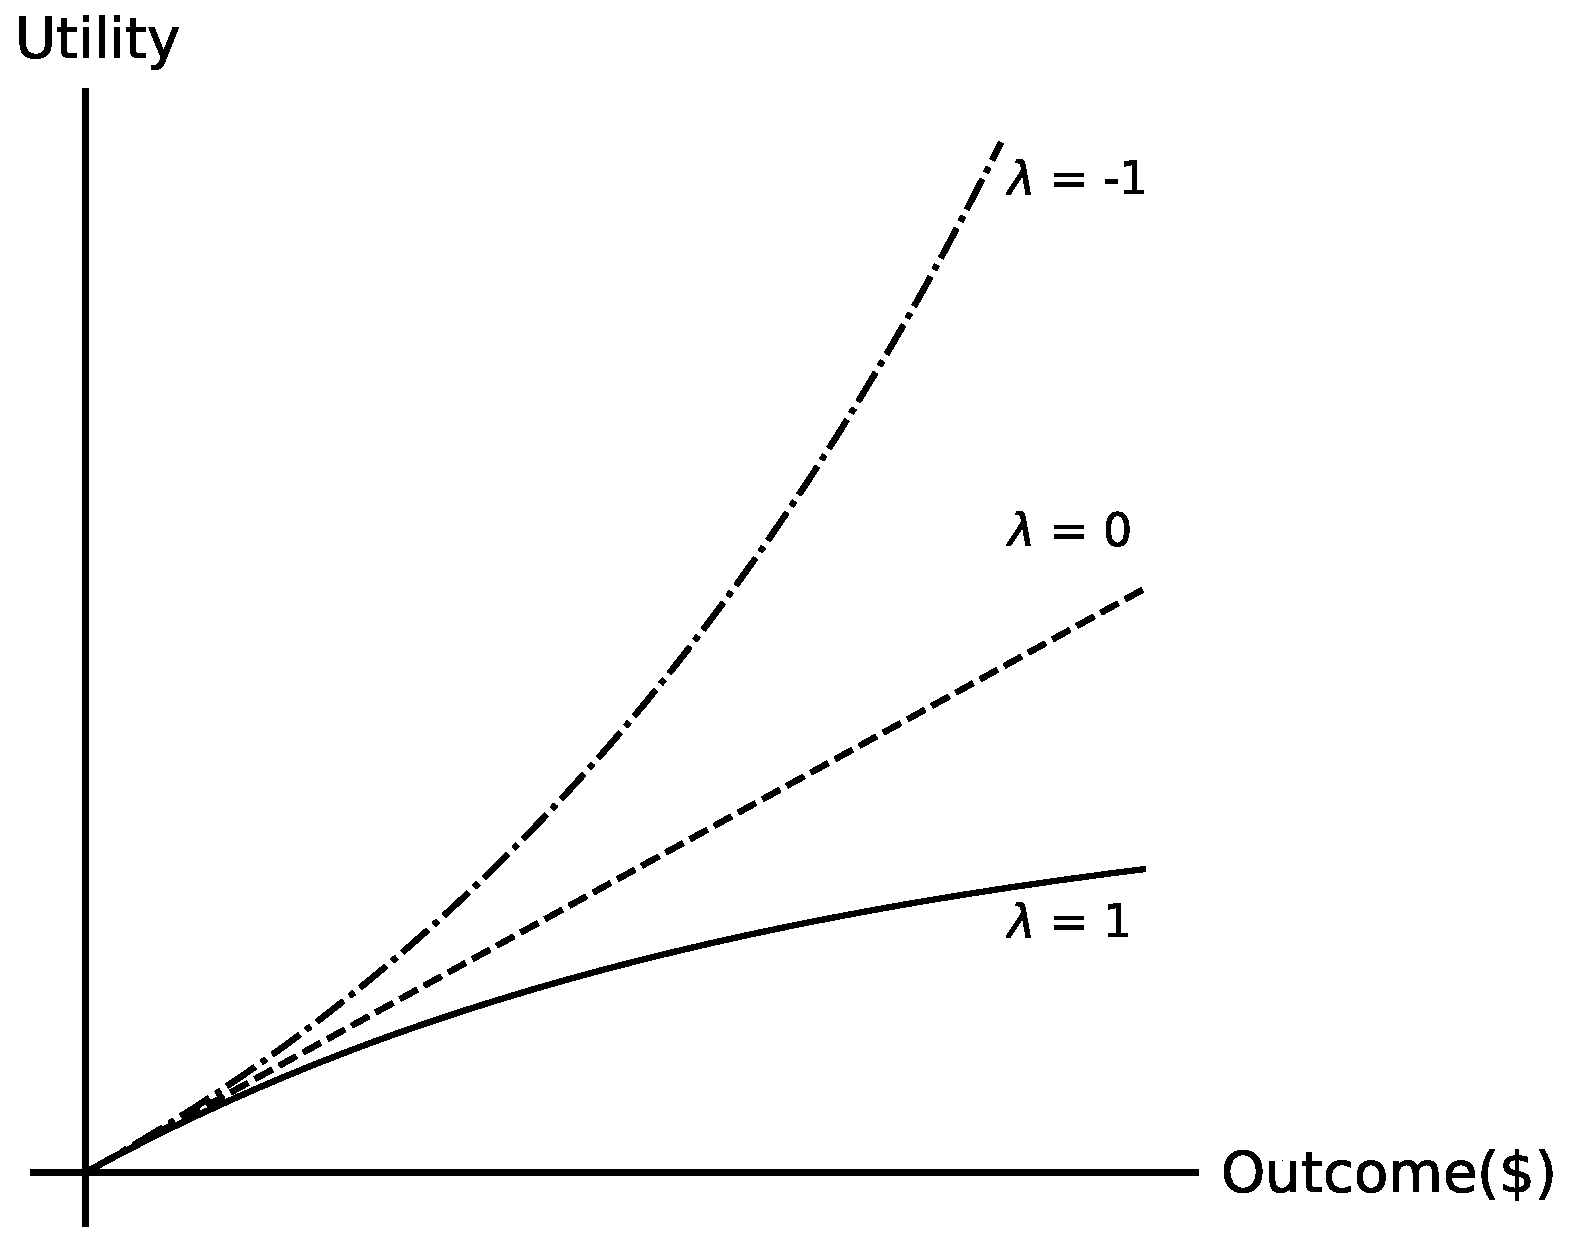
\includegraphics[width=0.3\textwidth]{img/background/Exponential_Utility_Function.pdf}%
\caption{ 
The exponential utility function for different risk parameters $\lambda$. $\lambda < 0$ implies risk seeking, $\lambda = 0 $ risk neutral and $\lambda > 0 $ risk averse behaviour.
}
\label{fig:background:exponential}
\end{figure}




% ###########################################################################

\subsection{Partially Observable Markov Decision Process}

Markov Decision Processes (MDPs) are a common choice for mathematically modelling risky decision making. Markov Decision Processes are usually defined over a finite state environment in which an agent can take actions with probabilistic outcomes that then affect the environment. At each time step the agent can fully observe in what state the environment is in.

Therefore an MDP is fully defined by the following four items:
\begin{itemize}
    \item Set of states $\mathcal{S}$ (terminal and non-terminal)
    \item Set of actions $\mathcal{A}$
    \item Probabilistic state transitions depending on tuple $\mathcal{S} \times \mathcal{A}$
    \item Reward function $R(s,a)$
\end{itemize}

To model decision making under uncertainty a MDP can be adopted to be partially observable instead. It is then called a Partially Observable Markov Decision Process (POMDP). In contrast to the classical MDP the agent no longer knows which state the environment is in. Instead it gets observations that it must use to infer the environments state.
This means the agent has to work on a probability distribution over states rather than the actual state.

To formally adopt the MDP framework we add two more items:
\begin{itemize}
    \item Observation space $\mathcal{O}$
    \item Observation function $p(o | s, a)$
\end{itemize}


A cartoon connecting all the pieces and showing the interactions between agent and environment can be seen in figure \ref{fig:background:agentenv}. The system is in a cyclical flow alternating between environment and agent. The agent performs an action that causes a state transition in the environment. The new state emits an observation and possibly a reward that are fed back to the agent. The agent uses this information to update its belief state and then acts according to its policy.

\begin{figure}
  \centering
    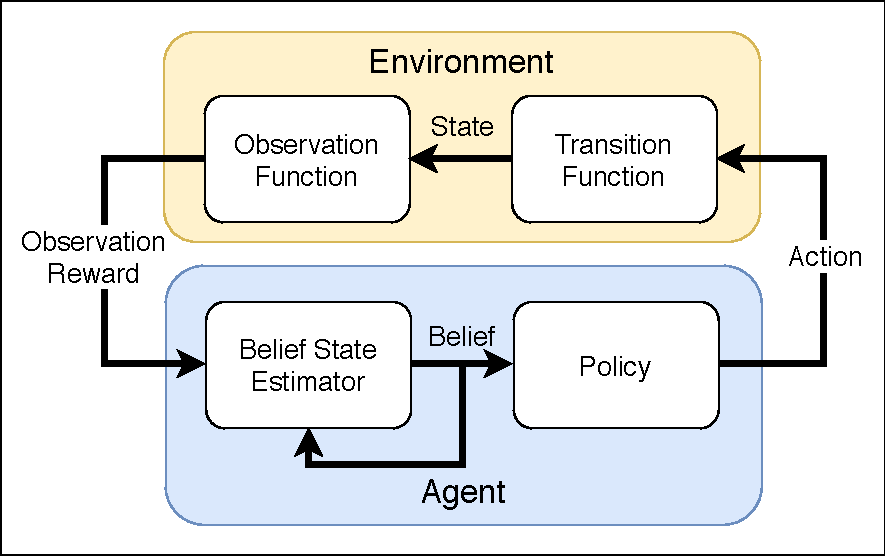
\includegraphics[width=0.5\textwidth]{img/background/POMDP}
  \caption{Sketch of a partially observable environment. The agent only gets observations and rewards as inputs but cannot see the state of the environment.}
  \label{fig:background:agentenv}
\end{figure}






% add reference: http://www.cassandra.org/arc/papers/aaai94.pdf

\section{Methods}\label{sec:methods}
\subsection{Experiment}

As a way to test our hypothesis we conducted a behavioral experiment to gather empirical data. We developed a web app where people could participate in a simulated investment task.

In the experiment people where told that they own a house that they want to sell. At the beginning of the simulation the housing market is in recession but when the participants wait long enough it will eventually change to a booming market and prices will increase. To introduce pressure on the participants they have to pay maintenance cost for every year they wait.
The goal then is to sell the house as soon as possible after the market has become booming.

The current state of the market is not directly observable by the participant. Instead at each time step one of the following things was shown to them:
\begin{itemize}
    \item Scenario 1: a price for which one of the houses in their neighborhood was sold, samples from a gaussian distribution with different mean depending on the market state.
    \item Scenario 2: the belief of an "expert" (the Bayesian estimate based on the observation history) that shows the chances of the market being in a good state
\end{itemize}

Given this information they had to infer in what state the market actually is and act accordingly.

~\autoref{fig:user-interface} shows how the interface of the experiment looks like for the two scenarios. In the first scenario, the participant was shown a new house price together with all the past observations in the form of a historic plot. In the second scenario they were given only the current belief. Besides this the interface constantly shows the total amount of money that the participant has spent on maintenance so far.

\begin{figure}[!htbp]
    \centering
    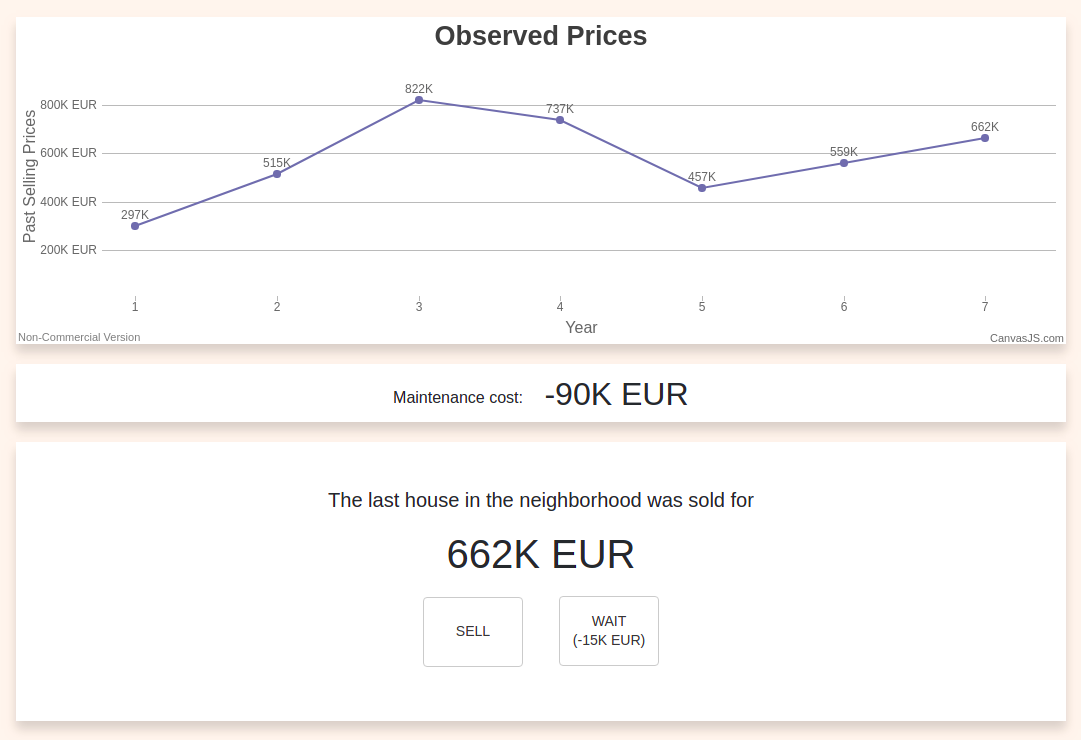
\includegraphics[width=0.99\linewidth]{img/methods/experiment_obs_1.png}\\
    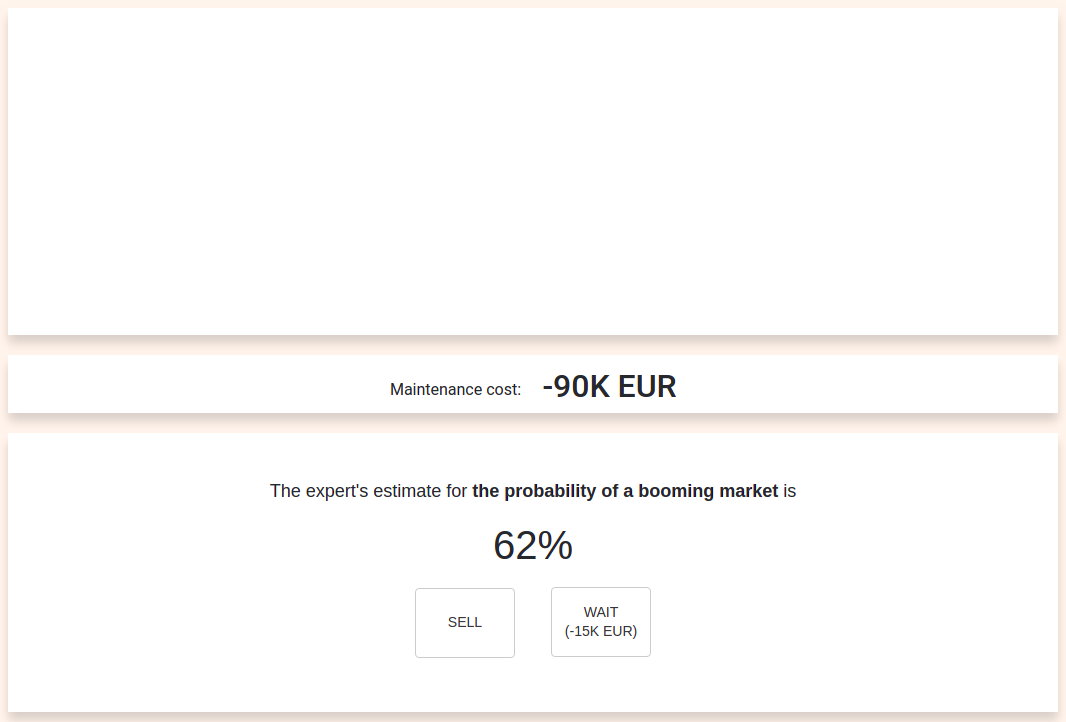
\includegraphics[width=0.99\linewidth]{img/methods/experiment_bel_1.png}\\
    \caption{The two experiment scenarios and their respective UI. In (a) subjects are shown the observation history at the top and a new observation at the bottom. In (b) they see the Bayesian estimate based on the observation history.}\label{fig:user-interface}
\end{figure}

~\autoref{fig:states} shows a graphical representation of the underlying environment. The market has three states, \textit{recession} and \textit{booming} and \textit{sold}. The market starts in recession in each experiment and iteratively transitions are performed. At each transition subjects are shown an observation from the current state and can choose between \textit{wait} and \textit{sell}. The experiments ends when subjects sell and they receive a reward based on the last market state.

\begin{figure}[H]
\tikzset{
scale=0.62, every node/.append style={transform shape}
}
\begin {center}
\begin {tikzpicture}[-latex ,auto ,node distance =3cm and 4cm ,on grid ,
semithick , scale=0.5, transform shape,
state/.style ={ circle ,fill=black!20, minimum width =3 cm}]
\node[state] (C){\large Sold};
\node[state] (A) [above left=of C,align=center] {\large Recession};
\node[state] (B) [above right =of C,align=center] {\large Booming};
\coordinate[below of=A] (AA);
\coordinate[below of=B] (BB);
\coordinate[below of=AA] (D);
\coordinate[below of=BB] (E);

\path (A) edge [loop left, line width=1mm, align=center] node[left] {\large wait \\ $\alpha =$ \\  $0.86$} (A);
\path (A) edge [bend left = -25,line width=1mm,align=center] node[below =0.25 cm] {\large sell\\$1.0$} (C);
\path (A) edge [bend left =25,line width=1mm,align=center] node[above] {\large wait\\$0.14$} (B);

\path (B) edge [loop right,line width=1mm,align=center] node[right] {\large wait\\$1.0$} (B);
\path (B) edge [bend right = -25,line width=1mm,align=center] node[below =0.25 cm] {\large sell\\$1.0$} (C);

%\fill[gray!40!white, opacity=0.5] (-6,-1) rectangle (5,6);

\path (A) edge [bend right =25,line width=1mm, dashed] node[left] {\large $Observation$} (D);
\path (B) edge [bend left  =25,line width=1mm, dashed] node[right] {\large $Observation$} (E);
\end{tikzpicture}
\end{center}
    \caption{Market States}\label{fig:states}
\end{figure}

The experiment was conducted with 24 participants and each one of them did the following runs:
\begin{itemize}
    \item 25 runs with random samples from the observations experiment with an easy setup (low maintenance costs.)
    \item 25 runs with random samples from the observations experiment with a hard setup (high maintenance costs.)
    \item 60 runs with random samples from the belief experiment.
\end{itemize}

The participants were paid according to their performance (average reward over all experiment runs) in order to give motivate them for performing as good as possible in the experiment.


\subsection{Solving the risk sensitive POMDP}
Marecki \cite{marecki} showed that RSPOMDPs can be solved for arbitrary utility functions using \keyword{reverse value iteration} in Belief Wealth Space.
For this the original state space must be augmented two times:

\begin{figure}[H]
\begin {center}
\begin {tikzpicture}[-latex ,auto ,node distance =3cm and 3cm ,on grid,
semithick , state/.style ={ circle ,fill=black!20, maximum width =2 cm}]
\node[state] (A) [align=center] {Observation\\Time\\Space};
\node[state] (B) [right of=A,align=center] {Belief\\Time\\Space};
\node[state] (C) [right of=B,align=center] {Belief\\Wealth\\Space};

\path (A) edge [line width=1mm, align=center] node[left] {} (B);
\path (B) edge [line width=1mm,align=center] node[below =0.25 cm] {} (C);
\end{tikzpicture}
\end{center}
\end{figure}

First augmentation is done by describing the probability of being in the good state with a function $\phi(b,o)$ ~\autoref{m:belief-update}:

\begin{align}
    b' = \phi(b,o) := ()
\end{align}

This augmentation transforms the POMDP into a MDP.
Second augmentation ...
\section{Results}\label{sec:results}
\subsection{Solving the risk sensitive POMDP}

\normalsize
Marecki \cite{marecki} showed that RSPOMDPs can be solved for arbitrary utility functions using \textbf{reverse value iteration} in Belief Wealth Space.
For this the original state space must be augmented two times:

\begin{figure}
\begin {center}
\begin {tikzpicture}[-latex ,auto ,node distance =4cm and 2cm ,on grid,
semithick , state/.style ={ circle ,fill=black!20, minimum width =3 cm}]
\node[state] (A) [align=center] {Observation\\Time\\Space};
\node[state] (B) [right of=A,align=center] {Belief\\Time\\Space};
\node[state] (C) [right of=B,align=center] {Belief\\Wealth\\Space};


\path (A) edge [line width=2mm, align=center] node[left] {} (B);
\path (B) edge [line width=2mm,align=center] node[below =0.25 cm] {} (C);
\end{tikzpicture}
\end{center}
\end{figure}

\hspace{2cm}

\subsection{Value functions in belief wealth space}


\normalsize

\begin{figure}
    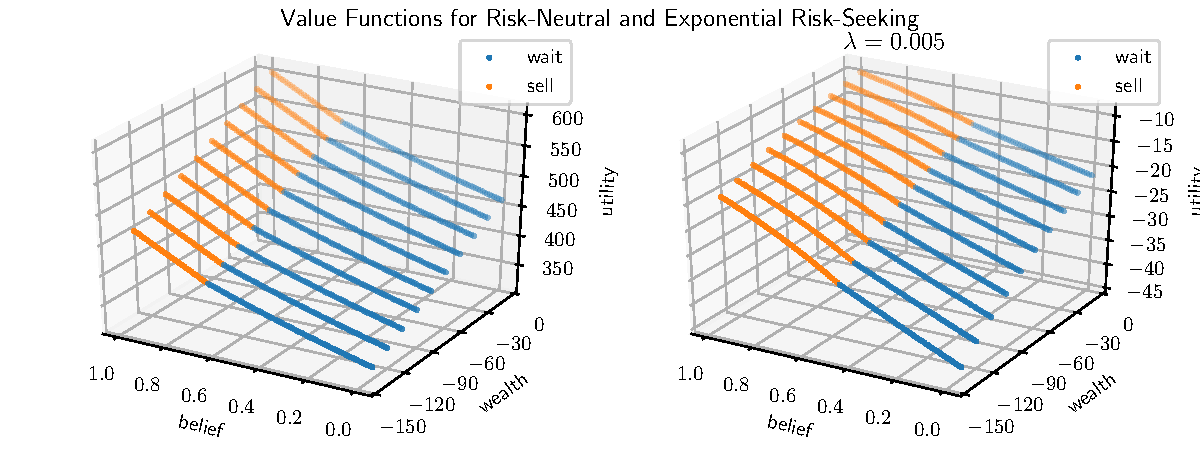
\includegraphics[width=0.98\linewidth]{img/exp_policy.pdf}\\
    \vspace{1cm}
    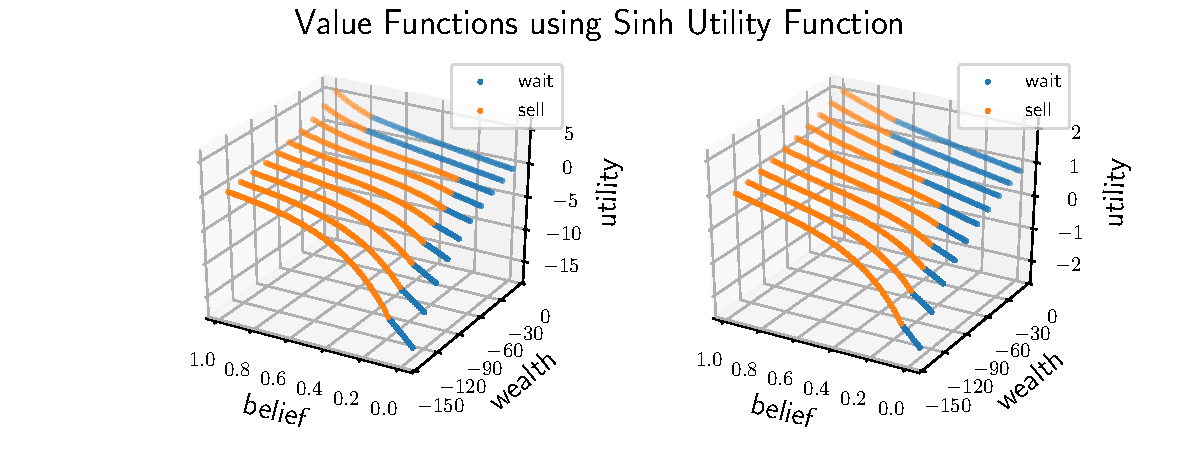
\includegraphics[width=0.98\linewidth]{img/sinh_policy.pdf}\\
    \vspace{1cm}
    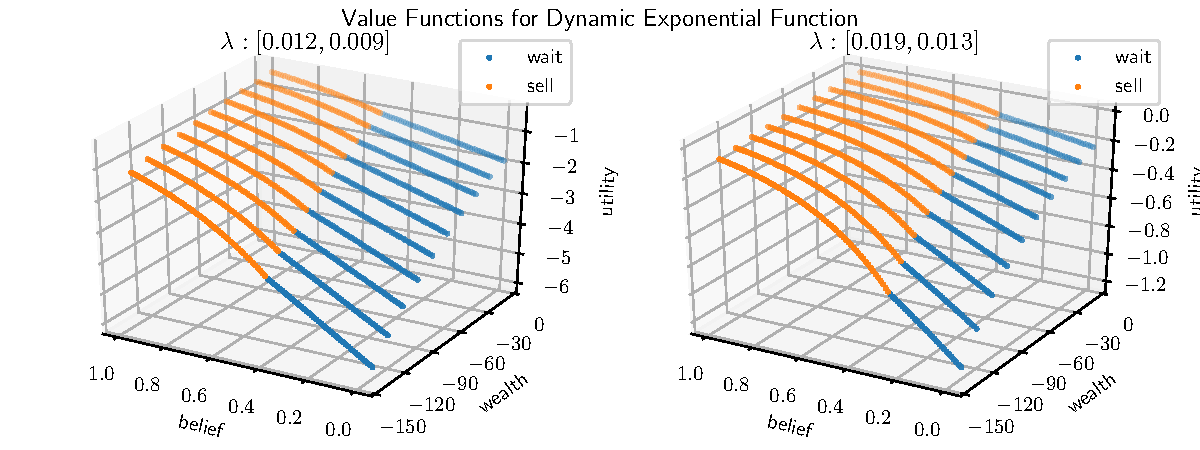
\includegraphics[width=0.98\linewidth]{img/dyn_policy.pdf}
    \caption{Value functions exhibiting different risk-behaviors; from top left: risk neutral agent (utility function is the identity function), risk-seeking agent with exponential utility function, two fixed time agents with different time thresholds, two agents with dynamic exponential utility function.}
\end{figure}

\subsection{From human behavior to utility functions}


\normalsize
\textbf{The original problem:}
\begin{itemize}
\item[①] Choose utility function with risk parameter.
\item[②] Perform value iteration.
\item[③] Derive policy.
\end{itemize}

\textbf{The inverse problem:}
\begin{itemize}
\item[①] Observe behavior.
\item[②] Estimate policy.
\item[③] Derive utility function and risk parameters.
\end{itemize}

The original problem is easy to solve, unfortunately for the inverse problem no solution is known. 

$\rightarrow$ Perform grid-search and choose optimal utility function.

\begin{figure}
    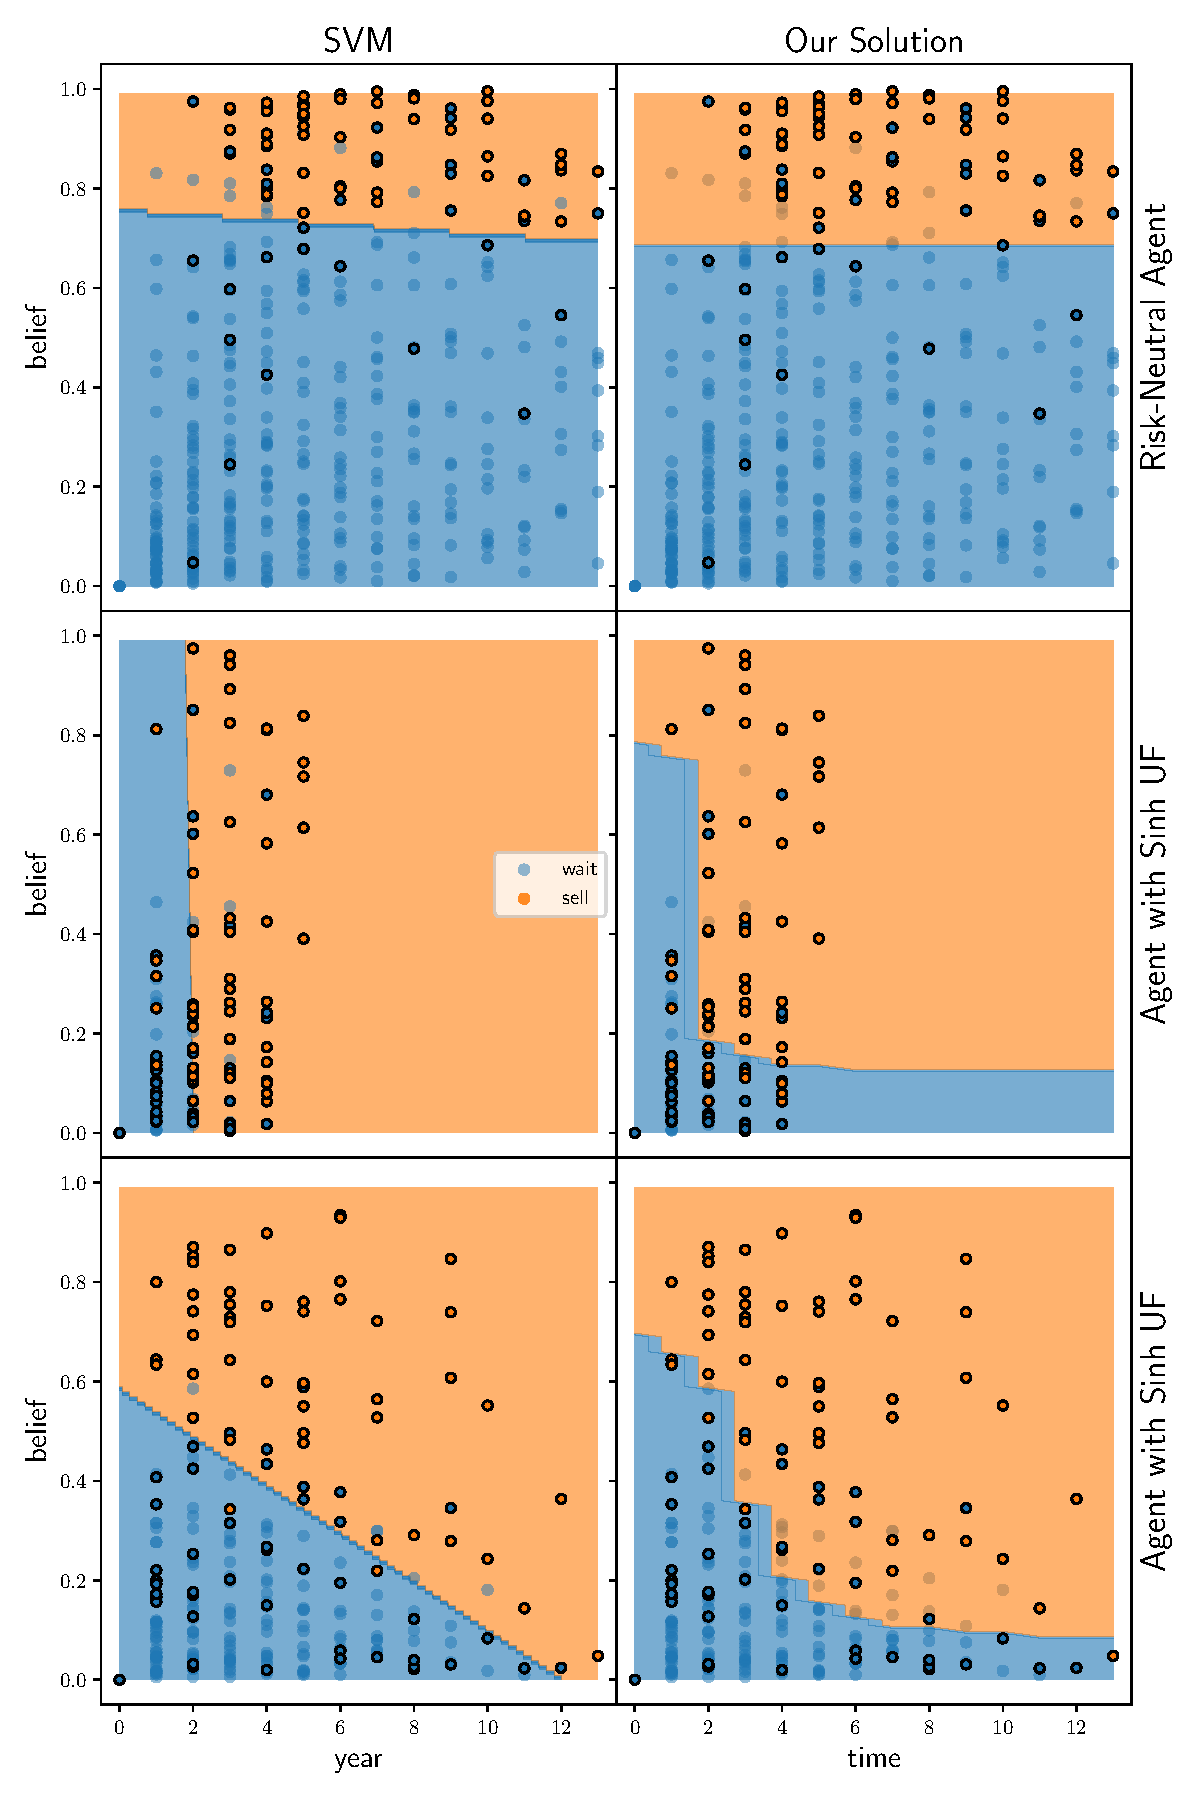
\includegraphics[width=0.8\linewidth]{img/fit}
    \caption{Examples from three human behaviors distinctly observed and replicated with RL agents. Behaviours by row: 1) Constant belief threshold, modelled by exponential utility, 2) Fixed time threshold, modelled by sinh utility, 3) Mixed strategy, modelled by dynamic exponential utility. Left column shows empirical optimal split of data using cross validation and linear kernel support vector machines, right column shows optimal policy found via gridsearch.}
    \label{fig:svm_vs_value}
\end{figure}

% TODO 6 boxes with only expensive expert and 3 behavior clusters.

\begin{figure}
% 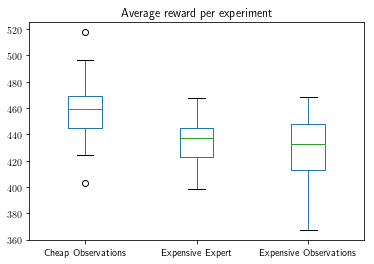
\includegraphics[width=0.4\linewidth]{img/avg_reward.png}
% 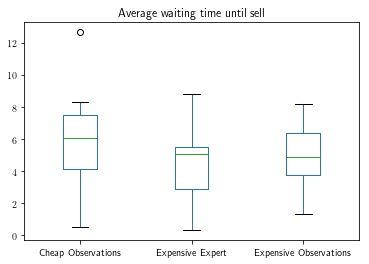
\includegraphics[width=0.4\linewidth]{img/avg_waiting.png}
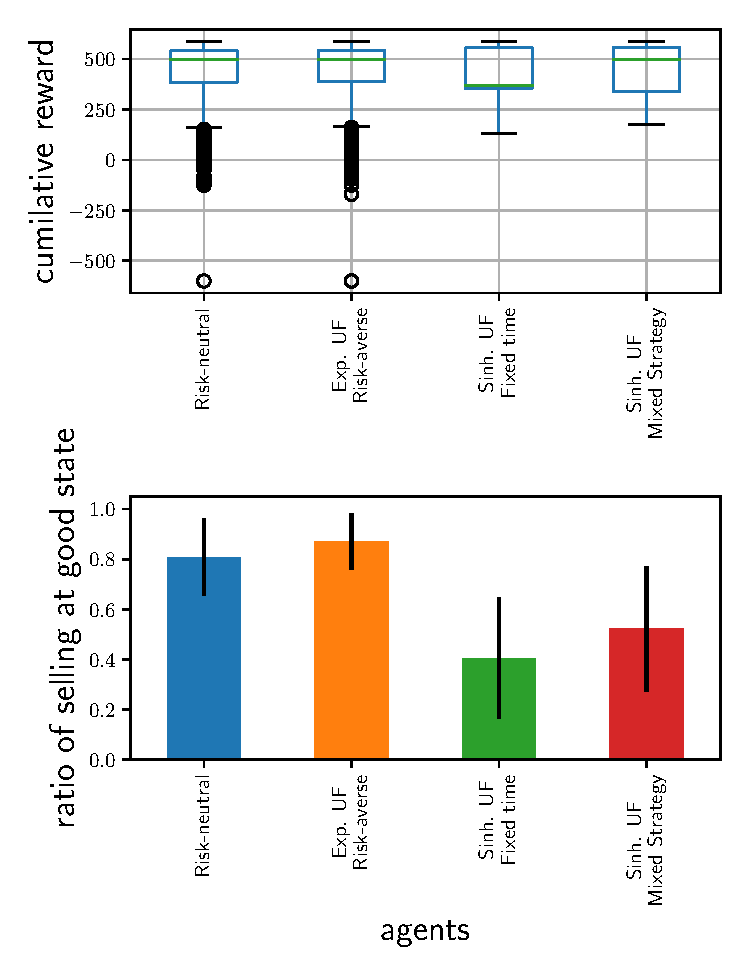
\includegraphics[width=0.8\linewidth]{img/performance.pdf}
\caption{Average reward and ratio of selling in the good state.}
\end{figure}

\section{Discussion}\label{sec:discussion}
Using the experimental data and reinforcement learning agents, we could provide evidence that the exponential utility function is not able to capture all human risk behaviour under uncertainty. While the EUF implies a time-independent policy, we found that the majority of our participants acted in a time-dependent manner. The parametrized $\text{sinh}$ utility function seems to explain these participants fairly well.

However, much work is left to be done. In particular, solving the inverse reinforcement learning problem to obtain utility function corresponding to risk-profiles in a more direct and accurate way.

% Acknowledgements should only appear in the accepted version.
\section*{Acknowledgements}

This work was supported by the NI Department. The authors gratefully acknowledge the helpful discussions and technical assistance provided by Rong Guo, Vaios Laschos and Robert Seidel.
We also thank the WZB department for assisting us during the execution of the experiment.


% In the unusual situation where you want a paper to appear in the
% references without citing it in the main text, use \nocite
\nocite{langley00}

\bibliography{example_paper}
\bibliographystyle{icml2018}


%%%%%%%%%%%%%%%%%%%%%%%%%%%%%%%%%%%%%%%%%%%%%%%%%%%%%%%%%%%%%%%%%%%%%%%%%%%%%%%
%%%%%%%%%%%%%%%%%%%%%%%%%%%%%%%%%%%%%%%%%%%%%%%%%%%%%%%%%%%%%%%%%%%%%%%%%%%%%%%
% DELETE THIS PART. DO NOT PLACE CONTENT AFTER THE REFERENCES!
%%%%%%%%%%%%%%%%%%%%%%%%%%%%%%%%%%%%%%%%%%%%%%%%%%%%%%%%%%%%%%%%%%%%%%%%%%%%%%%
%%%%%%%%%%%%%%%%%%%%%%%%%%%%%%%%%%%%%%%%%%%%%%%%%%%%%%%%%%%%%%%%%%%%%%%%%%%%%%%
\appendix
\section{Behavioral data for all subjects}
All of the behavioral data fitted with linear kernel support vector machine is shown in~\autoref{fig:all_beh}.


\begin{figure}
    \centering
    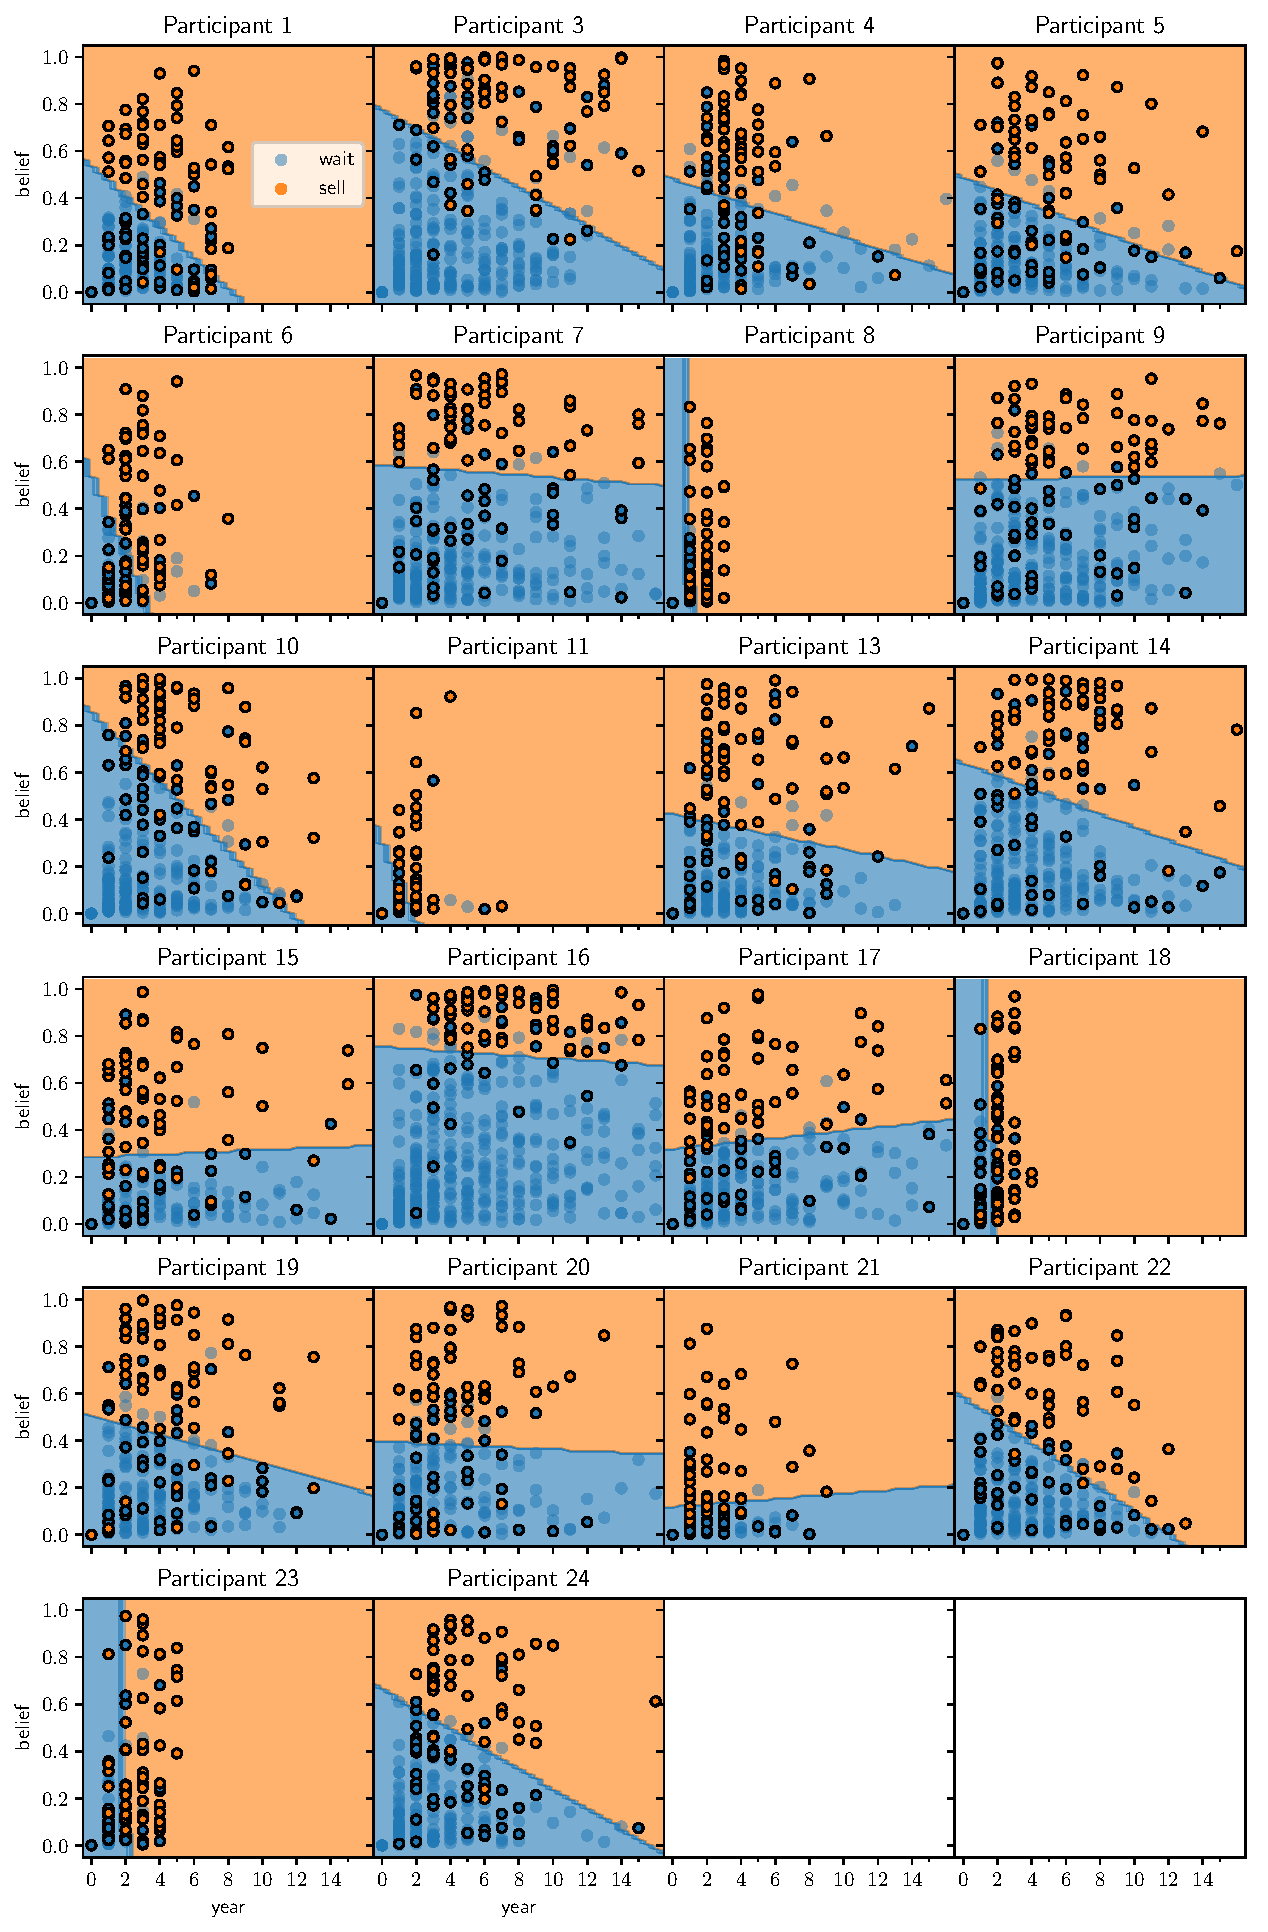
\includegraphics[width=0.99\linewidth]{img/all_peeps.pdf}
    \caption{All behavioral data collected and fitted with a linear kernel SVM. Participant 2 and 7 have been removed because of invalid behavior (they always sold at very first time step, which by definition is never booming.)}
    \label{fig:all_beh}
\end{figure}

\end{document}


% This document was modified from the file originally made available by
% Pat Langley and Andrea Danyluk for ICML-2K. This version was created
% by Iain Murray in 2018. It was modified from a version from Dan Roy in
% 2017, which was based on a version from Lise Getoor and Tobias
% Scheffer, which was slightly modified from the 2010 version by
% Thorsten Joachims & Johannes Fuernkranz, slightly modified from the
% 2009 version by Kiri Wagstaff and Sam Roweis's 2008 version, which is
% slightly modified from Prasad Tadepalli's 2007 version which is a
% lightly changed version of the previous year's version by Andrew
% Moore, which was in turn edited from those of Kristian Kersting and
% Codrina Lauth. Alex Smola contributed to the algorithmic style files.
